\subsubsection{Elliptic Curves Diffie Hellman key exchange}
The Diffie-Hellman key exchange (DH) is a key-agreement protocol used to generate a common secret between the two parts over an insecure channel; the computed secret is guaranteed to be the same for both and it's in the form of a byte array (in our case with length 32). From that secret then a deterministic key generation algorithm is able to extract a symmetric key usable for encryption/decryption. The Elliptic Curves DH (ECDH) works like this: every part computes a key pair over the same EC (we use the ones computed in the wizard), then both send their own public key to the other; now they multiply (for a proper definition on multiplication in a EC field) the public key of the other by their own private key: the result is the same due to the public/private EC keys mathematical properties as shown in the picture below.\\

\vspace{1cm}
\begin{center}
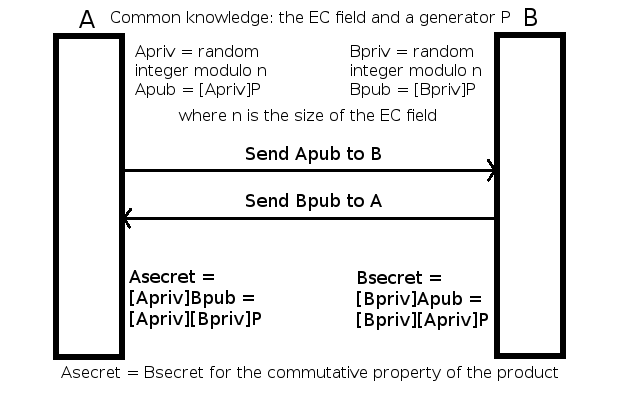
\includegraphics[scale=0.7]{images/ecdh}\\

\vspace{1cm}
Picture 1: ECDH schema\\
\end{center}

\vspace{1cm}
The problem with ECDH is the lack of authentication of the received public key: an active MITM could impersonate user A with user B and user B with user A by tricking them into believe his public key belongs to the other side while actually it's not true. This single point of failure is solved by embedding ECDH into SMP (see section 4.3.6).